\chapter{Integral de Riemann}

\section{Introducción}

\begin{quotation}
\marginnote{\adjustimage{max size={0.9\linewidth}{0.9\paperheight}}{imagenes/Riemann.jpeg}\\
Bernhard Riemann 1826-1866
} 
<< Bernard Riemann recibió su doctorado en 1851, su \emph{Habilitación} en 1854. La habilitación confiere el reconocimiento de la capacidad de crear sustanciales contribuciones en la investigación más allá de la tesis doctoral, y es un prerequisito necesario para ocupar un cargo de profesor en una universidad Alemana. Riemann eligió como tema  de habilitación el problema de las series de Fourier. Su tesis fue titulada \emph{\"Uber die Darstellbarkeit einer Function durch eine trigonometrische Reine} (Sobre la representación de una función por series trigonométricas) y respondía la pregunta:  Cuándo una función definida en el intervalo $(-\pi,\pi)$ puede ser respresentada por la serie trigonométrica $a_0/2+\sum_{n=1}^{\infty}[a_n\cos(nx)+b_n\sen(nx)]$? 
En este trabajo  es donde hallamos   la Integral de Riemann, introducida en una sección corta antes del nucleo principal de la tesis, como parte del trabajo preparatorio que él necesitó desarrollar antes de abordar el problema de representabilidad por series trigonométricas. >> 
\end{quotation}
\begin{flushright}
 David M. Bressoud\\
 A Radical Approach to Lebesgue's Theory of Integration.
\end{flushright}


En este capítulo vamos a desarrollar el concepto de la integral de Riemman. Vamos a exponer la definición de la integral debida a Riemann y la ideada por J. G. Darboux.
Mostraemos la equivalencia de las dos definiciones y discutiremos las propiedades de la intergal, sus alcances y límites. Preparamos así el camino para la introducción de la integral de Lebesgue. 
\marginnote{\adjustimage{max size={0.9\linewidth}{0.9\paperheight}}{imagenes/Darboux.jpg}\\
Jean G. Darboux  1842-1917
} 

Debemos advertir  al alumno que en este curso dejaremos un poco de lado las cuestiones procedimentales de cómo calcular integrales, aspecto que seguramente abordó en cursos anteriores y del cual nos vamos a valer. Tampoco debe esperar que las actividades prácticas se centren en esa dirección.   Nuestro principal objetivo aquí es discutir la materia conceptual ligada a la integral y cómo es previsible las actividades prácticas estarán orientadas con ese propósito.


El concepto de integral encuentra su motivación en diversos problemas. Aparece cuando se busca el centro de masas de un determinado cuerpo, cuando se quieren hallar longitudes de arco, volúmenes, cuando se quiere reconstruir el movimiento de cuerpo conocida su velocidad, etc. La integral es utilizada en incontables otros conceptos matemáticos, como ser el mencionado már arriba relativo a las series de Fourier. 

Quizás el 
problema más simple donde aparece la integral es el que utilizaremos como motivación para introducirla y es el concepto de área.  Vamos a tratar de reconstruir este concepto desde su base, esto es analizando la noción de área de figuras tan simples como rectángulos, triángulos, etc. 



\section{Área de figuras elementales planas}\label{sec:area_elem}

  
El cálculo de áreas es necesario en multitud de actividades humanas, por ejemplo con el comercio. La cantidad de muchos productos y servicios se estima en medidas de área, por ejemplo: las telas,  el trabajo de un colocador de pisos,  el precio de la construcción,  el valor de las extensiones de tierra, etc.  
 
 


Por figuras elementales planas nos referimos a rectángulos, triángulos, trapecios, etc. Sin duda el alumno  debe estar  muy familiarizado con las áreas de estas figuras, el área de un rectángulo viene dada por la conocida fórmula $b\times h$, donde $b$ es la base del rectángulo y $h$ su altura.  Ahora bien, ¿Cómo 
se llega a esta fórmula? Porque esta fórmula es apropiada para calcular el precio de un terreno por ejemplo. En esta sección vamos a justificar esta fórmula a partir de algunos hechos elementales.



Vamos a considerar un plano $\mathcal{P}$. En este plano $\mathcal{P}$ supondremos fijada una unidad de longitud.  Pretendemos asignar un área a las figuras, es decir a los subconjuntos, de $\mathcal{P}$. De ahora en más, cómo es usual en esta materia  nos referiremos a \emph{medida}\index{medida} en lugar de área. La medida es un concepto más general  que el concepto de área. No obstante en el contexto en que estamos actualmente son sinónimos.  

Queremos construir pues una función $m$ tal que $m(A)$ reppresente la medida  de  $A\subset\mathcal{P}$. Ahora bien ¿qué podemos usar de guía con ese objetivo? Si, como dijimos,  desconocemos todas las fórmulas previamente aprendidas, sobre que partimos para construir la medida o área. La respuesta es que tomaremos como principio rector  ciertas propiedades que son deseables  que una medida satisfaga. Ellas son las  siguientes. 




\begin{description}
 \item[Positividad.] debería ser una magnitud no negativa.  
 \item[Invariancia por movimientos rígidos.] Si una región es transformada en otra por medio de un movimiento rígido, ambas regiones deberían tener la misma área. Otra manera de expresar esta propiedad es diciendo que dos figuras \emph{congruentes}\index{congruencia} tienen la misma área. 
 \item[Aditividad.] Si una región es la unión de cierta cantidad de regiones más chicas mutuamente disjuntas  
\end{description}

\begin{figure}[h]
\begin{center}
 
\definecolor{xdxdff}{rgb}{0.49,0.49,1}
\definecolor{zzttqq}{rgb}{0.6,0.2,0}
\definecolor{ududff}{rgb}{0.30,0.30,1}
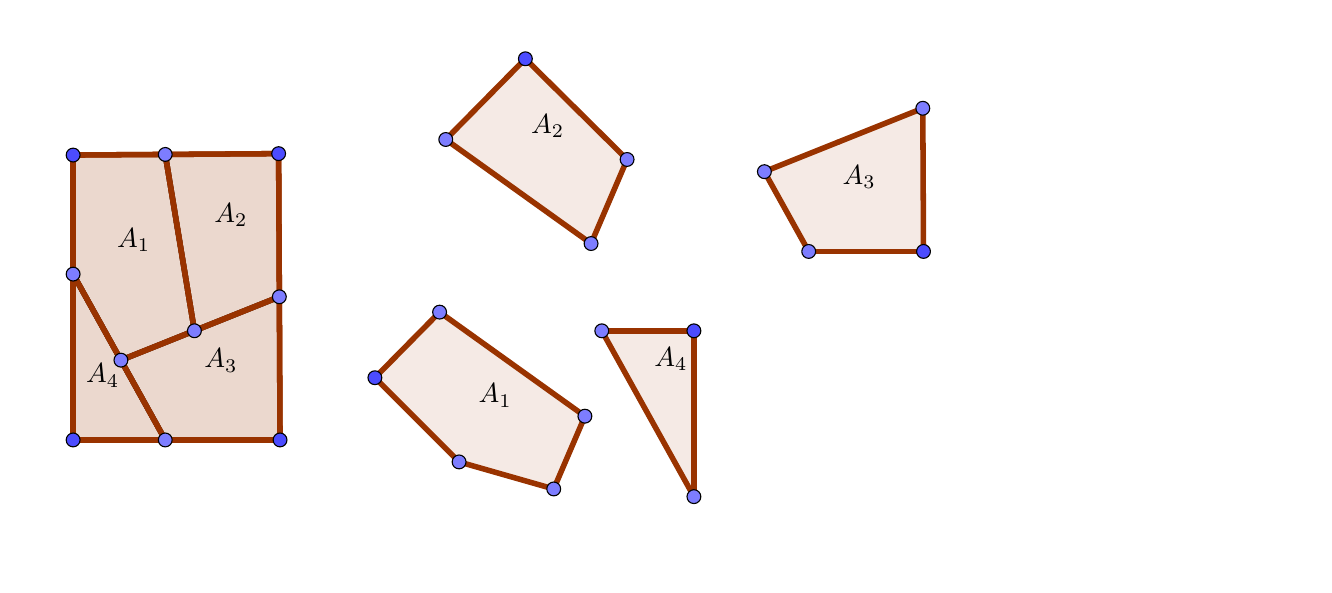
\begin{tikzpicture}[line cap=round,line join=round,x=.9cm,y=.9cm]
\clip(-2.261345665671131,-2.6483801457242535) rectangle (15.749723988011487,4.927708528477943);
\fill[line width=2pt,color=zzttqq,fill=zzttqq,fill opacity=0.10000000149011612] (-1.62,-0.89) -- (-1.62,3.13) -- (1.28,3.15) -- (1.3,-0.89) -- cycle;
\fill[line width=2pt,color=zzttqq,fill=zzttqq,fill opacity=0.10000000149011612] (0.09169246661626662,0.6507662540293884) -- (1.2899992647959808,1.130148511211861) -- (1.28,3.15) -- (-0.3199239037382289,3.1389660420431844) -- cycle;
\fill[line width=2pt,color=zzttqq,fill=zzttqq,fill opacity=0.10000000149011612] (-1.62,1.45) -- (-1.62,3.13) -- (-0.3199239037382289,3.1389660420431844) -- (0.09169246661626662,0.6507662540293884) -- (-0.9454716981132074,0.2358490566037732) -- cycle;
\fill[line width=2pt,color=zzttqq,fill=zzttqq,fill opacity=0.10000000149011612] (-1.62,-0.89) -- (-0.32,-0.89) -- (-1.62,1.45) -- cycle;
\fill[line width=2pt,color=zzttqq,fill=zzttqq,fill opacity=0.10000000149011612] (-0.32,-0.89) -- (-0.9454716981132074,0.2358490566037732) -- (0.09169246661626662,0.6507662540293884) -- (1.2899992647959808,1.130148511211861) -- (1.3,-0.89) -- cycle;
\fill[line width=2pt,color=zzttqq,fill=zzttqq,fill opacity=0.10000000149011612] (8.76,1.77) -- (8.134528301886792,2.8958490566037733) -- (9.171692466616268,3.3107662540293887) -- (10.36999926479598,3.790148511211861) -- (10.38,1.77) -- cycle;
\fill[line width=2pt,color=zzttqq,fill=zzttqq,fill opacity=0.10000000149011612] (3.8264466094067267,-1.199878066911803) -- (2.6385072170133266,-0.011938674518402692) -- (3.551459891609421,0.9136938983359697) -- (5.601939561385962,-0.5546723179904587) -- (5.16194451123264,-1.5814488960049211) -- cycle;
\fill[line width=2pt,color=zzttqq,fill=zzttqq,fill opacity=0.10000000149011612] (5.6888024763961145,1.8814084921516754) -- (6.19715889449669,3.0677137999207305) -- (4.761837661840736,4.4888939366884495) -- (3.638322806619573,3.3497747084781038) -- cycle;
\fill[line width=2pt,color=zzttqq,fill=zzttqq,fill opacity=0.10000000149011612] (7.14,0.65) -- (5.84,0.65) -- (7.14,-1.69) -- cycle;
\draw [line width=2pt,color=zzttqq] (-1.62,-0.89)-- (-1.62,3.13);
\draw [line width=2pt,color=zzttqq] (-1.62,3.13)-- (1.28,3.15);
\draw [line width=2pt,color=zzttqq] (1.28,3.15)-- (1.3,-0.89);
\draw [line width=2pt,color=zzttqq] (1.3,-0.89)-- (-1.62,-0.89);
\draw [line width=2pt] (-1.62,1.45)-- (-0.32,-0.89);
\draw [line width=2pt] (-0.9454716981132074,0.2358490566037732)-- (1.2899992647959808,1.130148511211861);
\draw [line width=2pt] (-0.3199239037382289,3.1389660420431844)-- (0.09169246661626662,0.6507662540293884);
\draw [line width=2pt,color=zzttqq] (0.09169246661626662,0.6507662540293884)-- (1.2899992647959808,1.130148511211861);
\draw [line width=2pt,color=zzttqq] (1.2899992647959808,1.130148511211861)-- (1.28,3.15);
\draw [line width=2pt,color=zzttqq] (1.28,3.15)-- (-0.3199239037382289,3.1389660420431844);
\draw [line width=2pt,color=zzttqq] (-0.3199239037382289,3.1389660420431844)-- (0.09169246661626662,0.6507662540293884);
\draw [line width=2pt,color=zzttqq] (-1.62,1.45)-- (-1.62,3.13);
\draw [line width=2pt,color=zzttqq] (-1.62,3.13)-- (-0.3199239037382289,3.1389660420431844);
\draw [line width=2pt,color=zzttqq] (-0.3199239037382289,3.1389660420431844)-- (0.09169246661626662,0.6507662540293884);
\draw [line width=2pt,color=zzttqq] (0.09169246661626662,0.6507662540293884)-- (-0.9454716981132074,0.2358490566037732);
\draw [line width=2pt,color=zzttqq] (-0.9454716981132074,0.2358490566037732)-- (-1.62,1.45);
\draw [line width=2pt,color=zzttqq] (-1.62,-0.89)-- (-0.32,-0.89);
\draw [line width=2pt,color=zzttqq] (-0.32,-0.89)-- (-1.62,1.45);
\draw [line width=2pt,color=zzttqq] (-1.62,1.45)-- (-1.62,-0.89);
\draw [line width=2pt,color=zzttqq] (-0.32,-0.89)-- (-0.9454716981132074,0.2358490566037732);
\draw [line width=2pt,color=zzttqq] (-0.9454716981132074,0.2358490566037732)-- (0.09169246661626662,0.6507662540293884);
\draw [line width=2pt,color=zzttqq] (0.09169246661626662,0.6507662540293884)-- (1.2899992647959808,1.130148511211861);
\draw [line width=2pt,color=zzttqq] (1.2899992647959808,1.130148511211861)-- (1.3,-0.89);
\draw [line width=2pt,color=zzttqq] (1.3,-0.89)-- (-0.32,-0.89);
\draw [line width=2pt,color=zzttqq] (8.76,1.77)-- (8.134528301886792,2.8958490566037733);
\draw [line width=2pt,color=zzttqq] (8.134528301886792,2.8958490566037733)-- (9.171692466616268,3.3107662540293887);
\draw [line width=2pt,color=zzttqq] (9.171692466616268,3.3107662540293887)-- (10.36999926479598,3.790148511211861);
\draw [line width=2pt,color=zzttqq] (10.36999926479598,3.790148511211861)-- (10.38,1.77);
\draw [line width=2pt,color=zzttqq] (10.38,1.77)-- (8.76,1.77);
\draw [line width=2pt,color=zzttqq] (3.8264466094067267,-1.199878066911803)-- (2.6385072170133266,-0.011938674518402692);
\draw [line width=2pt,color=zzttqq] (2.6385072170133266,-0.011938674518402692)-- (3.551459891609421,0.9136938983359697);
\draw [line width=2pt,color=zzttqq] (3.551459891609421,0.9136938983359697)-- (5.601939561385962,-0.5546723179904587);
\draw [line width=2pt,color=zzttqq] (5.601939561385962,-0.5546723179904587)-- (5.16194451123264,-1.5814488960049211);
\draw [line width=2pt,color=zzttqq] (5.16194451123264,-1.5814488960049211)-- (3.8264466094067267,-1.199878066911803);
\draw [line width=2pt,color=zzttqq] (5.6888024763961145,1.8814084921516754)-- (6.19715889449669,3.0677137999207305);
\draw [line width=2pt,color=zzttqq] (6.19715889449669,3.0677137999207305)-- (4.761837661840736,4.4888939366884495);
\draw [line width=2pt,color=zzttqq] (4.761837661840736,4.4888939366884495)-- (3.638322806619573,3.3497747084781038);
\draw [line width=2pt,color=zzttqq] (3.638322806619573,3.3497747084781038)-- (5.6888024763961145,1.8814084921516754);
\draw [line width=2pt,color=zzttqq] (7.14,0.65)-- (5.84,0.65);
\draw [line width=2pt,color=zzttqq] (5.84,0.65)-- (7.14,-1.69);
\draw [line width=2pt,color=zzttqq] (7.14,-1.69)-- (7.14,0.65);
\draw (-1.1356538123159674,2.2366014415507594) node[anchor=north west] {$A_1$};
\draw (3.9651373981996176,0.03798454046645946) node[anchor=north west] {$A_1$};
\draw (0.23628313396063827,2.5883801457242477) node[anchor=north west] {$A_2$};
\draw (4.703872676963944,3.83719454554013) node[anchor=north west] {$A_2$};
\draw (0.09557165229124281,0.5304747263093427) node[anchor=north west] {$A_3$};
\draw (9.101106479132552,3.1160482019844795) node[anchor=north west] {$A_3$};
\draw (-1.5753771925328282,0.31940750380524985) node[anchor=north west] {$A_4$};
\draw (6.445177262622713,0.5480636615180171) node[anchor=north west] {$A_4$};
\begin{scriptsize}
\draw [fill=ududff] (-1.62,-0.89) circle (2.5pt);
\draw [fill=ududff] (-1.62,3.13) circle (2.5pt);
\draw [fill=ududff] (1.28,3.15) circle (2.5pt);
\draw [fill=ududff] (1.3,-0.89) circle (2.5pt);
\draw [fill=xdxdff] (-1.62,1.45) circle (2.5pt);
\draw [fill=xdxdff] (-0.32,-0.89) circle (2.5pt);
\draw [fill=xdxdff] (-0.9454716981132074,0.2358490566037732) circle (2.5pt);
\draw [fill=xdxdff] (1.2899992647959808,1.130148511211861) circle (2.5pt);
\draw [fill=xdxdff] (-0.3199239037382289,3.1389660420431844) circle (2.5pt);
\draw [fill=xdxdff] (0.09169246661626662,0.6507662540293884) circle (2.5pt);
\draw [fill=xdxdff] (8.76,1.77) circle (2.5pt);
\draw [fill=xdxdff] (8.134528301886792,2.8958490566037733) circle (2.5pt);
\draw [fill=xdxdff] (10.36999926479598,3.790148511211861) circle (2.5pt);
\draw [fill=ududff] (10.38,1.77) circle (2.5pt);
\draw [fill=xdxdff] (3.8264466094067267,-1.199878066911803) circle (2.5pt);
\draw [fill=ududff] (2.6385072170133266,-0.011938674518402692) circle (2.5pt);
\draw [fill=xdxdff] (3.551459891609421,0.9136938983359697) circle (2.5pt);
\draw [fill=xdxdff] (5.601939561385962,-0.5546723179904587) circle (2.5pt);
\draw [fill=xdxdff] (5.16194451123264,-1.5814488960049211) circle (2.5pt);
\draw [fill=xdxdff] (5.6888024763961145,1.8814084921516754) circle (2.5pt);
\draw [fill=xdxdff] (6.19715889449669,3.0677137999207305) circle (2.5pt);
\draw [fill=ududff] (4.761837661840736,4.4888939366884495) circle (2.5pt);
\draw [fill=xdxdff] (3.638322806619573,3.3497747084781038) circle (2.5pt);
\draw [fill=ududff] (7.14,0.65) circle (2.5pt);
\draw [fill=xdxdff] (5.84,0.65) circle (2.5pt);
\draw [fill=xdxdff] (7.14,-1.69) circle (2.5pt);
\end{scriptsize}
\end{tikzpicture}


 \caption{El área del rectángulo es la suma de sus partes}\label{fig:rect_descop} 
\end{center}
\end{figure}

Utilizando la segunda y tercer propiedad se pueden relacionar el área del rectángulo de la figura \ref{fig:rect_descop} con las cuatro regiones en la que es dividido.

Como veremos a lo largo de la materia la propiedad de aditividad debe ser estudiada con cuidado, esto ocurre por las intrincadas maneras en que una región puede ser unión de otras regiones. A lo largo de esta materia elaboraremos una  teoría que nos dará una descripción  precisa de a que conjuntos podemos asignarle una medida de modo que las propiedades previas sean ciertas. 

Por el momento veamos como las propiedades anteriores determinan practicamente de manera unívoca la medida de regiones elementales planas.  


Hablando de propiedades de la medida, supongamos que $A$ y $B$ son dos regiones con $A\subset B$. Entonces como $B=A\cup (B-A)$ y por la propiedad de aditividad y positividad

\[
 m(B)=m(A)+m(B-A)\geq m(A).
\]

Descubrimos así que nuestra medida deberá tener adicionalmente la siguiente propiedad:
\begin{description}
 \item[Monotonía.] Si $A\subset B$ entonces $m(A)\leq m(B)$. 
\end{description}
\marginpar{ Podríamos por ejemplo elegir el círculo de radio uno como unidad de área. Así ya no tendríamos el problema de ese número raro $\pi$ que aparece en la fórmula del área del círculo. ¡El área de cualquier círculo sería igual a su radio al cuadrado! Claro que aparecería $\pi$  en la fórmula del área del cuadrado de lado 1. Nos tapamos los pies y se destapa el cuerpo.}
Es claro que si logramos construir una medida que satisfaga las propiedades anteriores cualquier multiplo por un número real positivo  de ella seguirá cumpliendo las propiedades. Esto es una manera de expresar el hecho que podemos usar diferentes unidades de medición. Esta cuestión se sortea proponiendo la unidad de medida. Esta unidad es completamente arbitraria, ud. podría elegir su figura plana preferida como unidad de área.   Cómo es habitual, elijamos el cuadrado cuyos lados miden la unidad de longitud previamente fijada. 


Supongamos ahora que tenemos un rectángulo de un lado igual a la unidad y el otro de lado un racional $n/m$, $n,m\in\mathbb{N}$. Veamos que la aditividad, la invariancia por movimientos rígidos y el hecho que decidimos que el cuadrado de lados igual a la unidad determinan el área de este rectángulo. Primero observar que si dividimos el lado de cuadrado unidad en $m$ segmentos iguales de longitud. \marginnote{
 
\definecolor{xdxdff}{rgb}{0.49,0.49,1}
\definecolor{zzttqq}{rgb}{0.6,0.2,0}
\definecolor{ududff}{rgb}{0.30,0.30,1}
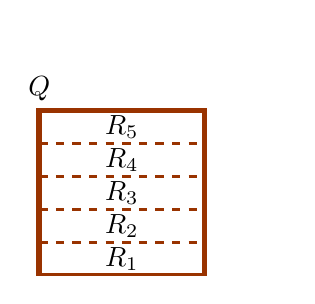
\begin{tikzpicture}[x=2.1cm,y=2.1cm]
\clip(-0.07,0) rectangle (1.5,1.5);
\draw [line width=2pt,color=zzttqq] (0,0) -- (1,0) -- (1,1) -- (0,1) -- cycle;
\draw [line width=1pt,color=zzttqq, dashed] (0,.2)--(1,.2);
\draw [line width=1pt,color=zzttqq, dashed] (0,.4)--(1,.4);
\draw [line width=1pt,color=zzttqq, dashed] (0,.6)--(1,.6);
\draw [line width=1pt,color=zzttqq, dashed] (0,.8)--(1,.8);
\draw (0,1) node[anchor=south] {$Q$};
\draw (0.5,.1) node[anchor=center] {$R_1$};
\draw (0.5,.3) node[anchor=center] {$R_2$};
\draw (0.5,.5) node[anchor=center] {$R_3$};
\draw (0.5,.7) node[anchor=center] {$R_4$};
\draw (0.5,.9) node[anchor=center] {$R_5$};



\end{tikzpicture}
\\
 Descomposición rectángulo $R$
 }
Queda dividido el cuadrado en $m$ rectángulos $R_1,\ldots,R_m$ (ver figura en el margen), todos ellos  congruentes entre si, de modo que todos tienen la misma medida, digamos $m(R_1)$. La unión de ellos es el cuadrado que por convención dijimos que tiene medida 1. De modo que por la aditividad debe ocurrir que $m(R_1)=\cdots =m(R_m))=1/m$. Recordemos nuestra pretención de inferir la medida de un rectángulo $R$ de lado 1 y otro $n/m$. Este rectángulo esta compuesto de $n$ rectángulos congruentes a los $R_i$, $i=1,\ldots,m$, nuevamente por la aditividad inferimos que $m(R)=n/m$. 

Sea ahora una rectángulo $R$ con un lado unidad y el otro un real cualquiera $l>0$. Existen sendas sucesiones $0<q_k,p_k\in\mathbb{Q}$, $k\in\mathbb{N}$, tales que $q_1\leq q_2\leq\cdots \leq l \leq \cdots\leq p_2\leq p_1$ y $\lim_{k\to\infty}q_k =\lim_{k\to\infty} p_k=l$. Consideremos una dos sucesiones de rectángulos $R_k$ y $S_k$ que comparten el lado de $R$ igual a la unidad, mientras que el otro lado de $R_k$ y $S_k$ es igual a $q_k$ y $p_k$ respectivamente. Luego por la monotonía
\[
 q_k=m(R_k)\leq m(R) \leq m(S_k)\leq p_k.
\]
Tomando límite cuando $k\to\infty$ inferimos que $m(R)=l$. 



\begin{figure}[h]
 \begin{center}
 \input{imagenes/ParalTria.tikz} 
 \end{center}
 \caption{Áreas de otras figuras elementales.}\label{fig:paral-trig}
\end{figure}


A partir de las propiedades fundamentales que postulamos para la medida o área inferimos la famosa fórmula del área de un rectángulo en el caso que uno de los lados sea igual a la unidad. Para un  rectángulo arbitrario. En la figura \ref{fig:paral-trig} se muestra como relacionar el área de un paralelepípedo con la de un rectángulo y la de un triángulo con la de un paralelepípedo para inferir las conocidas fórmulas para estas figuras.



\section{Integral de Riemann}

En esta sección abordaremos el problema del área de regiones planas. Vamos a contextualizarnos dentro del marco conceptual que nos brinda la geometría analítica. Mediante coordenadas cartesianas ortogonales los puntos del plano se identifican con pares ordenados $(x,y)\in\mathbb{R}^2$ y el plano con el conjunto $\rr^2$.  Nuestro propósito es entonces definir la medida de subconjuntos de $\mathbb{R}^2$. La geometría analítica abre así nuevas posibilidades para abordar el problema del área. 

Nuestra primera aproximación será la que propuso Bernhard Riemann en 1854, pero seguiremos  el enfoque de Jean Darboux. En esta parte de nuestra exposición consideraremos subconjuntos de $\mathbb{R}^2$ de un tipo especial, concretamente a conjuntos que quedan encerrados entre la gráfica de una función y del eje coordenadas $x$. Esto nos lleva alconcepto de integral. 


\begin{definicion}[Partición]{} Sea $[a,b]$ un intervalo. Una {\em partición}\index{Partición} $P$ es un conjunto ordenado y finito de puntos, donde el primer elemento es $a$ y el último $b$. Es decir $P=\{x_0,x_1,\ldots,x_n\}$, donde $a=x_0<x_1<\cdots<x_n=b$. 
 
\end{definicion}




\begin{definicion}[Sumas de Darboux]{} Sea $f:[a,b]\to\mathbb{R}$ una función acotada y $P=\{x_0,x_1,\ldots,x_n\}$ una partición de $[a,b]$. Consideremos las siguientes magnitudes
\[
 \begin{split}
    m_i&:=\inf\{f(x)| x\in [x_{i-1},x_i]\}\\
    M_i&:=\sup\{f(x)| x\in [x_{i-1},x_i]\}\\
 \end{split}
\]

Definimos la \emph{Suma superior de Darboux}\index{Suma superior} como
\[
 \overline{S}(P,f)=\sum_{i=1}^nM_i(x_i-x_{i-1}),
\]
y la \emph{Suma inferior de Darboux}\index{Suma inferiorr} como
\[
 \underline{S}(P,f)=\sum_{i=1}^nm_i(x_i-x_{i-1}),
\] 
\end{definicion}
\marginpar{
  \begin{center}
    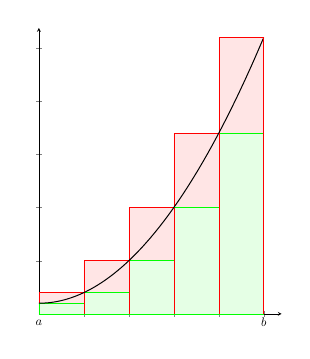
\begin{tikzpicture}[scale=0.45]
\begin{axis}[
    xtick={0,...,5},ytick={5,10,15,20,25},
    y=0.3cm, xmax=5.4,ymax=26.9,ymin=0,xmin=0,
    enlargelimits=true,
    axis lines=middle,
    clip=false,yticklabels=\empty,xticklabels=\empty,
    ]
\addplot+[color=red,fill=red!10!white,const plot, mark=none]
    coordinates {(0,2) (1,5) (2,10) (3,17) (4,26) (5,26)}\closedcycle;
\addplot+[color=green,fill=green!10!white,const plot, mark=none]
    coordinates {(0,1) (1,2) (2,5) (3,10) (4.0,17) (5,17)}\closedcycle;
\addplot[smooth, thick,domain=0:5]{1+x^2};
\addplot[const plot,domain=0:5,color=red] coordinates {(1,0) (1,2)};
\addplot[const plot,domain=0:5,color=red] coordinates {(2,0) (2,5)};
\addplot[const plot,domain=0:5,color=red] coordinates {(3,0) (3,10)};
\addplot[const plot,domain=0:5,color=red] coordinates {(4,0) (4,17)};
\addplot[const plot,domain=0:5,color=red] coordinates {(5,0) (5,26)};
\addplot[color=black] coordinates {(0,-0.8)} node {$a$};
\addplot[color=black] coordinates {(5,-0.8)} node {$b$};

\end{axis}
\end{tikzpicture}
    Sumas de Darboux. 
  \end{center}
}

\begin{lema}[Monotonía sumas de Darboux]{}  Sea $f:[a,b]\to\mathbb{R}$ una función acotada y $P=\{x_0,x_1,\ldots,x_n\}$ una partición de $[a,b]$. Supongamos que $P'$ es otra partición que tiene un pnto más que $P$. Entoces
 \[
  \underline{S}(P',f)\geq \underline{S}(P,f)\quad\text{y}\quad \overline{S}(P',f)\leq \overline{S}(P,f)
 \]
\end{lema}

\begin{ejercicio}{} Sea $f:[a,b]\to\mathbb{R}$ una función acotada y $P,P'$ particiones de $[a,b]$ con $P\subset P'$. Demostrar que 
  \[
  \underline{S}(P,f)\leq \underline{S}(P',f)\quad\text{y}\quad \overline{S}(P',f)\leq \overline{S}(P,f).
 \]
 Inferir que para cualesquiera $P,P'$ (sin importar que una este o no contenida dentro de la otra)
   \[
\underline{S}(P,f)\leq \overline{S}(P,f).
 \]
 
\end{ejercicio}

\begin{definicion}[Funciones integrables]{} Sea $f:[a,b]\to\mathbb{R}$ una función acotada. Diremos que $f$ es {\em integrable Riemann} \index{Integrable Riemann} si 
\begin{equation}\label{eq:integrable}
 \sup\left\{\underline{S}(P,f)| P \text{partición de }[a,b]\right\}=\inf\left\{\overline{S}(P,f)| P \text{partición de }[a,b]\right\}
\end{equation}
En caso que $f$ sea integrable llamamos {\em integral} \index{Integral} entre $a$ y $b$ de $f$ al valor de los dos miembros de \eqref{eq:integrable} y este número se denota
\[
\int_a^bf(x)dx. 
\]
 
\end{definicion}
 
\begin{teorema}[Primer criterio de integrabilidad]{}  Sea $f:[a,b]\to\mathbb{R}$ una función acotada. Entonces  $f$ sea integrable si para todo $\epsilon>0$ existe una partición $P$ tal que 
\begin{equation}\label{eq:Crit1Int}
 \overline{S}(P;f)-\underline{S}(P;f)<\epsilon.
\end{equation}
 
\end{teorema}

\begin{demo} La demo
 
\end{demo}


\begin{ejemplo}{} Sea $0\leq a<b$ veamos que 
\[
 \int_a^b x dx=\frac{b^2}{2}-\frac{a^2}{2}.
\]
\end{ejemplo}


\begin{ejercicio}{} Sea $0\leq a<b$ veamos que 
\[
 \int_a^b x^2 dx=\frac{b^3}{3}-\frac{a^3}{3}.
\]
{\em Ayuda:} Usar particiones uniformes y la fórmula $\sum_{i=1}^nn^2= n(n+1)(2n+1)/6$.
\end{ejercicio}

\begin{ejemplo}{} Sea $0\leq a<b$ y $n\in\mathbb{N}$,  veamos que 
\[
 \int_a^b x^n dx=\frac{b^{n+1}}{n+1}-\frac{a^{n+1}}{n+1}.
\]
Usamos particiones no uniformes
\end{ejemplo}

\begin{ejercicio}{} Sea $0\leq a<b$ y $n$ un entero negativo, veamos que
\[
 \int_a^b x^n dx=\begin{cases}
                  \frac{b^{n+1}}{n+1}-\frac{a^{n+1}}{n+1} & \text{ si } n\neq -1\\
                  \ln(b)-\ln(a) & \text{ si } n=-1\\
                 \end{cases}
\]
\end{ejercicio}


\begin{ejemplo}{} Sea $0\leq a<b\leq \pi/2$, veamos que
\[
 \int_a^b \sen x dx=-(\cos(b)-\cos(a)).
\]
\end{ejemplo}



\begin{ejercicio}{} Sea $0\leq a<b\leq \pi$, veamos que
\[
 \int_a^b \sen x dx=-(\cos(b)-\cos(a)).
\]
\end{ejercicio}


\begin{ejemplo}{} Usamos SymPy y sumas de Darboux aproximar el valor de $\pi$. Utilizamos el hecho que $\pi/4$ es el área de un cuarto de círculo de radio $1$. Entonces 
$$\pi=4\int_0^1\sqrt{1-x^2}dx.$$

\begin{sympyblock}
from sympy import *
N=1000.0
lim=int(N+1)
x=symbols('x')
f=sqrt(1-x**2)
Sinf=sum([ f.subs(x,i/N)*1/N for i in range(1,lim)])
Ssup=sum([f.subs(x,(i-1)/N)*1/N for i in range(1,lim)])
\end{sympyblock}
Encontramos la estimación
\[\sympy{4*Sinf}\leq \pi \leq \sympy{4*Ssup}\]
\end{ejemplo}

\begin{ejercicio}{} Usando SymPy estimar las siguientes integrales 
$$\int_1^2\frac{1}{x}dx,$$
 comparar con $\ln(2)$,

$$\int_{-1}^{1}x^2dx$$
¿A qué parece aproximarse las sumas inferiores y superiores?

$$\int_0^{\frac{1}{2}}\frac{1}{\sqrt{1-x^2}}dx,$$
¿Por qué el resultado puede usarse para aproximar $\pi$ ?

 
\end{ejercicio}




\begin{teorema}[Propiedades elementales de la integral]{} Sean $f,g:[a,b]\to\mathbb{R}$ integrables, $\alpha,\beta\in\mathbb{R}$ y $c\in (a,b)$. Entonces
\begin{description}
 \item[Linealidad] $\alpha f+\beta g$ es integrable y 
 \[
  \int_a^b\alpha f(x)+\beta g(x)dx=\alpha \int_a^bf(x)dx+\beta\int_a^b g(x)dx.
 \]
 \item[Monotonía] Si $f(x)\leq g(x)$  para $x\in [a,b]$ entonces 
 \[
  \int_a^b f(x)dx\leq \int_a^b g(x)dx.
 \]
 \item[Aditividad del Intervalo]  \[
  \int_a^b\alpha f(x)dx= \int_a^cf(x)dx+\int_c^b f(x)dx.
 \]
\end{description}


\end{teorema}

\begin{observa} Las propiedadades anteriores son compatibles con las propiedades que habíamos propuesto para el concepto de área en la sección  \ref{sec:area_elem}.
\end{observa}

\section{Integrabilidad y continuidad}


 
\begin{teorema}[Segundo criterio de integrabilidad]{}  Sea $f:[a,b]\to\mathbb{R}$ una función acotada. Entonces  $f$ sea integrable si para todo $\epsilon>0$ existe un $\delta>0$ tal que para cualquier partición $P$ que satisface
\[\max_i\{x_i-x_{i-1}\}<\delta,\]
se tiene que
\begin{equation}\label{eq:Crit1Int}
 \overline{S}(P;f)-\underline{S}(P;f)<\epsilon.
\end{equation}
 
\end{teorema}
\begin{demo} Agarrate catalina
 
\end{demo}

\begin{teorema}[Continuidad implica integrabilidad]{}  Si $f:[a,b]\to\mathbb{R}$ es una función continua entonces es integrable.
\end{teorema}
\begin{demo} hacer
 \end{demo}

 
¿Qué ocurre con las funciones discontinuas? 

\begin{ejemplo}[Función de Heavside]{} Es la función
\[
 H(x)=\begin{cases}0 & \text{ si } x<0\\1 & \text{ si } x\geq 0\end{cases}.
\]
Es discontinua en $[-1,1]$ pero integrable.
 
\end{ejemplo}



\marginnote{\adjustimage{max size={0.9\linewidth}{0.9\paperheight}}{imagenes/dirichlet.png}\\
Función de Dirichlet}
\begin{ejemplo}[Función de Dirichlet]{} Es la función $f:[0,1]\to\mathbb{R}$ definida por 
\[
 f(x)=\begin{cases} 1 & \text{ si } x\in\mathbb{Q}\\0 & \text{ si }   x\notin\mathbb{Q}\\
\end{cases}
\]
Veamos que $f$ es discontinua en todo punto y no integrable.
\end{ejemplo}





\begin{ejemplo}[Función de Thomae]{} Es la función $f:[0,1]\to\mathbb{R}$ definida por 
\[
 f(x)=\begin{cases} \frac{1}{q} & \text{ si } x=\frac{p}{q},p,q\in\mathbb{Z}, \text{m.c.d}(p,q)=1
 \\0 & \text{ si }   x\notin\mathbb{Q}\\
\end{cases}
\]
\end{ejemplo}
\marginnote{\adjustimage{max size={0.9\linewidth}{0.9\paperheight}}{imagenes/thomae.png}\\
Función de Thomae}

Para graficarla

\begin{sympyverbatim}
from matplotlib import pyplot as plt
total=500
q=[]
f=[]
for i in range(1,total):
    for j in range(1,i):
        if gcd(j,i)==1:
            q.append(Rational(j,i))
            f.append(1.0/i)
plt.plot(q,f,'.',markersize=12)
\end{sympyverbatim}

Veamos que es discontinua en todo punto racional y es integrable integrable.

\marginnote{\adjustimage{max size={0.9\linewidth}{0.9\paperheight}}{imagenes/escalera.png}\\
Función creciente y discontinua en $\mathbb{Q}\cap [0,1]$}
\begin{ejemplo}[Escalera discontinua]{} Sea $\mathbb{Q}\cap [0,1]=\{q_1,q_2,\ldots\}$ una numeración de los racionales del $[0,1]$. Definamos $f:[0,1]\to\mathbb{R}$ como
 \[
  f(x)=\sum_{n=1}^{\infty}H(x-q_n),
 \]
donde $H$ es la función de \emph{Heavside}\index{Heavside}. 
\begin{sympyverbatim}
q=[]
f=[]
total=20
for i in range(1,total):
    for j in range(1,i):
        if gcd(j,i)==1:
            q.append(float(Rational(j,i)))
x=symbols('x')
Heavside=Piecewise((0,x<0),(1,x>=0))
f=sum([Heavside.subs(x,x-q[n])/2**n for n in range(len(q))])
plot(f,(x,0,1))
\end{sympyverbatim}

Veamos que $f$ es monotona no decreciente y discontinua en todo punto de $[0,1]\cap \mathbb{Q}$. Además $f$ es integrable.


\end{ejemplo}
\begin{definicion}[Oscilación sobre un intervalo]{} Sea $f:[a,b]\to\mathbb{R}$ acotada y $I=[\alpha,\beta]\subset [a,b]$. Definimos la \emph{oscilación}\index{oscilación} de $f$ en $I$ por 
\[
 w(f,I)=\sup\{f(x)| x\in I\}-\inf\{f(x)| x\in I\}.
\]
\end{definicion}

\begin{ejemplo}{} 
\begin{enumerate}
 \item Para la función de Dirichlet $w(f,I)=1$ para todo $I$ con interior no vacío.
 \item Para la función de Heavside e $I=[\alpha,\beta]$
 \[
  w(f,I)=\begin{cases}
          1 & \text{ si } 0\in (\alpha,\beta]\\
          0 & \text{ si } 0\notin (\alpha,\beta]\\
         \end{cases}
 \]
  \item Si $I^o\neq\emptyset$, $f$ la función de Thomae e $I\subset [0,1]$ entonces 
     $ w(f,I)=1/q^*$, donde $q^*$ es el mínimo valor de $q$ para el que existe $p\leq q$ tal que $p/q\in I$.
  \item Para la función escalera discontinua e $I\subset [0,1]$
  \[
   w(f,I)=\sum_{q_n\in I}\frac{1}{2^n}.
  \]
\end{enumerate}

 
\end{ejemplo}



\begin{definicion}{} Sea $f:[a,b]\to\mathbb{R}$ acotada, $\sigma>0$ y $P=\{x_0,x_1,\ldots,x_n\}$ una partición. Definimos
\[
 I_{\sigma}:=\{i\in\{1,\ldots,n\}|w(f,[x_{i-1},x_i])>\sigma\}.
\]
y
\[
 R(P,f,\sigma)=\sum_{i\in I_{\sigma}}(x_i-x_{i-1}).
\]
\end{definicion}





\begin{proposicion} Si $f$ es continua en $[a,b]$ para todo $\sigma>0$ existe $\delta>0$ tal que 
\[
\max_i(x_i-x_{i-1})<\delta\Rightarrow I_{\sigma}=\emptyset\Rightarrow R(P,f,\sigma)=0. 
\]

 
\end{proposicion}

\begin{ejemplo}{} Para la función de Dirichlet y para todo $0<\sigma<1$ y para toda partición de $[0,1]$ tenemos $I_{\sigma}=\{x_1,\ldots,x_n\}$ y $R(P,f,\sigma)=[0,1]$
 
\end{ejemplo}

\begin{ejemplo}{} Para la función de Heavside,   para todo $0<\sigma<1$ y para toda partición de $[0,1]$ tenemos $I_{\sigma}=i$, donde $i$ es el índice para el que $i\in (x_{i-1},x_i]$ y $R(P,F,\sigma)=x_i-x_{i-1}$.
 
\end{ejemplo}

\begin{teorema}[Criterio de integrabilidad de Riemann]{} Sea $f$ acotada en $[a,b]$ entonces $f$ es integrable si y sólo si  para todo $\epsilon>0$ y $\sigma>0$ existe $\delta>0$ talque $R(P,f,\sigma)<\epsilon$.
\end{teorema}

\begin{ejemplo}{} Discutir los ejemplos Dirichlet, Heavside, Continuas, escalera discontinua
 
\end{ejemplo}

\begin{ejemplo}[Función de Riemann]{} Definimos
\[
 ((x))=x-[x+0.5]
\]

\marginnote{\adjustimage{max size={0.9\linewidth}{0.9\paperheight}}{imagenes/serrucho.pdf}\\
Función serrucho}
\begin{sympyverbatim}
x=symbols('x')
g=x-floor(x+.5)
plot(g,(x,-5,5))
\end{sympyverbatim}
Definimos la función de Riemann Porque
\[
 f(x)=\sum_{n=1}^{\infty}\frac{((x))}{n^2}.
\]

\begin{sympyverbatim}
f=sum([g.subs(x,n*x)/n**2 for n in range(1,20)])
plot(f,(x,0,1))
\end{sympyverbatim}
\marginnote{\adjustimage{max size={0.9\linewidth}{0.9\paperheight}}{imagenes/funcRiemann.png}\\
Función de Riemann}
 
Demostramos que la función de Riemann es discontinua en los racionales $p/q$ donde $\text{m.c.d}(p,q)=1$ y $q$ par. Es integrable en $[0,1]$.  
 
\end{ejemplo}


\begin{definicion}[Oscilación de una función en un punto]{}\index{oscilación} 
Sea $f:[a,b]\to\mathbb{R}$ y $x\in [a,b]$ 
acotada definimos la {\em oscilación de $f$ en $x$} como 
\[
 w(f;x)=\inf\limits_{x\in I^o}w(f,I),
\]
donde el ínfimo se toma sobre todos los intervalos que contienen a $x$ en su interior.
\end{definicion}

\begin{ejercicio}{} $f$ es continua en $x$ si y solo si $w(f;x)=0$.
 \end{ejercicio}

 \begin{definicion}[Contenido exterior]{}\index{Contenido exterior} Sea $S\subset\mathbb{R}$. Un \emph{cubrimiento finito}\index{cubrimiento finito} de $S$ es una colección de intervalos $\left\{ [x_{i-1},x_i]\right\}_{i=1,\ldots,n}$ tal que $S\subset \cup_{i=1}^n[x_{i-1},x_i]$.
 
 El \emph{contenido exterior} de $S$ se define por 
 \[
  c_e(S)=\inf \sum_{i=1}^n (x_i-x_{i-1}),
 \]
donde el ínfimo es tomado sobre todos los cubrimientos finitos de $S$.
  
 \end{definicion}
 
 \begin{teorema}[Criterio de integrabilidad de Hankel]{}  Sea $f$ acotada en $[a,b]$ entonces $f$ es integrable si y sólo si para todo $\sigma>0$ el conjunto $S_{\sigma}:=\{x\in [a,b]| w(f,x)>\sigma\}$ tiene contenido exterior igual a $0$ ($c_e(S_{\sigma})=0)$.
   \end{teorema}


\section{Teorema Fundamental de Cálculo}


\section{Función de Volterra}

\begin{pyblock}
import numpy as np
import scipy.optimize
from matplotlib import pyplot as plt
\end{pyblock}

Consideramos  la función $f(x)=x^2\sen(1/x)$. 

\begin{pyblock}
def G(x):
    return x**2*np.sin(1/x)
x=np.arange(0,.15,0.0000001)
y=G(x)
plt.plot(x,y)
\end{pyblock}


 \begin{figure}[h]
 \begin{center}
\adjustimage{max size={0.9\linewidth}{0.9\paperheight}}{imagenes/VolterraPrecursora.png}
 \caption{Función precursora de Volterra}
\end{center}
 \end{figure}





\begin{pyblock}
def F(x):
    return 2*x*np.sin(1/x) - np.cos(1/x)
x = scipy.optimize.broyden2(F, .13, f_tol=1e-14)
x,1-x, G(x)
\end{pyblock}

Se alcanza un máximo en $x=\py{np.float32(x)}$ y toma el valor $G(x)=\py{np.float32(G(x))}$. Hay que utilizar el punto simétrico a $x$, es decir $1-x=\py{np.float32(1-x)}$.


Definimos la función ``madre''.



\begin{pyblock}
def f0(x):
    x1=x[x<=0]
    x2=x[(x<=0.13163877)*(x>0)]
    x3=x[(x>0.13163877)*(x<0.868361226)]
    x4=x[(x>=0.868361226)*(x<1)]
    x5=x[x>=1]
    y1=np.zeros(np.shape(x1))
    y2=x2**2*np.sin(1/x2)
    y3=0.01675771541054875*np.ones(np.shape(x3))
    y4=(1-x4)**2*np.sin(1/(1-x4))
    y5=np.zeros(np.shape(x5))
    return np.concatenate((y1,y2,y3,y4,y5), axis=None)
\end{pyblock}

Definimos la función de Volterra
\begin{pyverbatim}
def volterra(x,n,a=0,b=1):
    if n == 0:
        return 0
    
    a1,b1 = 2.*a/3. + b/3., a/3. + 2.*b/3.
    pto_med = .5*(a+b)
    return volterra(x,n-1,a,a1) + (b1-a1)*f0((x-a1)/(b1-a1))\
    + volterra(x,n-1,b1,b)
\end{pyverbatim}

Graficamos

\begin{pyverbatim}
x=np.arange(0,1,0.0000001)
y=volterra(x,12)
plt.plot(x,y)
\end{pyverbatim}


 \begin{figure}[h]
 \begin{center}
\adjustimage{max size={0.9\linewidth}{0.9\paperheight}}{imagenes/volterra.png}
 \caption{Función de Volterra}
\end{center}
 \end{figure}


\section{Integral de Riemann y pasos al límite}

